\subsection{L'explorateur de fichiers}

\begin{figure}[h]
\begin{center}
    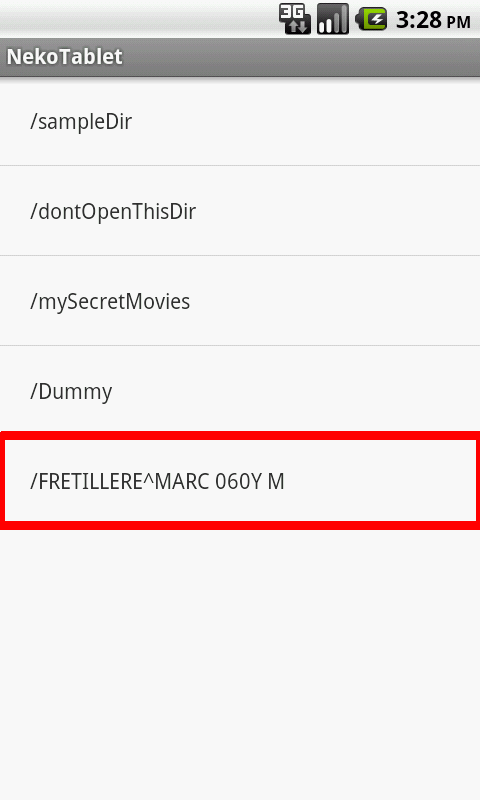
\includegraphics[width=12cm]{file-browser}
\end{center}
    \caption{Capture d'écran de l'explorateur de fichiers}
    \label{fichiers}                      
\end{figure}

L'ouverture de l'application conduit sur l'écran d'exploration des fichiers, visible en figure \vref{fichiers}.
Nous distinguons les dossiers normaux des dossiers \emph{DICOM}. Sur la figure \vref{fichiers}, on peut voir qu'un dossier a été entouré en rouge : il s'agit d'un exemple de dossier \emph{DICOM}. Ces derniers représentent un examen et contiennent les fichiers qui constituent les données de l'examen. Le nom du dossier \emph{DICOM} est masqué à l'utilisateur, qui voit à la place le nom, le prénom, le genre et l'âge du patient associé à l'examen.
Un clic sur un dossier quelconque place la vue à l'intérieur du dossier. On peut revenir dans le dossier parent par autre clic. Un clic sur un dossier \emph{DICOM} déclenche l'ouverture de l'examen et l'utilisateur passe alors sur l'affichage présenté dans le chapitre suivant.